\usetikzlibrary {shapes.geometric}
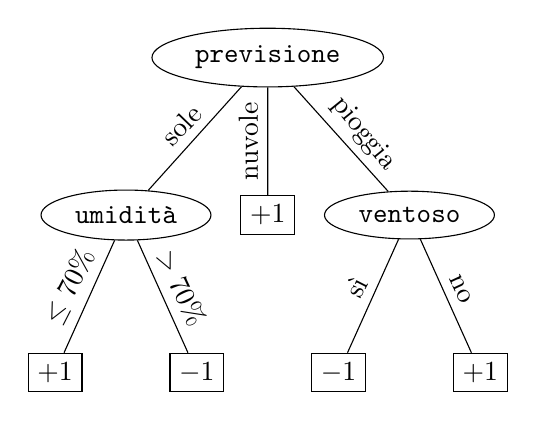
\begin{tikzpicture}[sibling distance=18mm, level distance=20mm]
    
    \node [ellipse,draw] {\texttt{previsione}}
        child {node[ellipse,draw] {\texttt{umidità}}
            child {node[rectangle,draw] {$+1$} edge from parent node[above,rotate=63] {$\leq 70\%$}}
            child {node[rectangle,draw] {$-1$} edge from parent node[above,rotate=-65] {$> 70\%$}}
            edge from parent node[above,rotate=46] {sole}
        }
        child {node[rectangle,draw] {$+1$} edge from parent node[above,rotate=90] {nuvole}}
        child {node[ellipse,draw] {\texttt{ventoso}} 
            child {node[rectangle,draw] {$-1$} edge from parent node[above,rotate=63] {sì}}
            child {node[rectangle,draw] {$+1$} edge from parent node[above,rotate=-65] {no}}
            edge from parent node[above,yshift=-.3em,xshift=.2em,rotate=-51] {pioggia}
        };

\end{tikzpicture}